\chapter{Estado del arte}\label{arte}
En el marco del desarrollo del desafío de Sistemas Expertos, se planteó generar un dispositivo de monitoreo a distancia de pacientes. Para esto se comenzó a estudiar aspectos relacionados con la Telemedicina y sus implicancias en el avance del monitoreo Remoto de Paciente (RPM, por sus siglas en inglés). La Telemedicina es, en principio, la tecnología que permite entregar cuidados médicos a través de la infraestructura de las telecomunicaciones, permitiendo a los médicos diagnosticar o evaluar enfermedades sin la necesidad de un control presencial.
Para poder comprender en qué se encuentra la realidad nacional y latinoamericana es de suma importancia revisar algunos casos dónde se apliquen dispositivos de telemedicina bajo la modalidad de monitorear y digitalizar la información, considerando que el objetivo del proyecto se limita a esas dos acciones.

\section{ViSi Mobile\textregistered}
ViSi Mobile\textregistered\ \cite{visi}, si bien se utiliza en el cuerpo, es una estación que procesa los datos de otros sensores que van colocados en el cuerpo y que a su vez se conectan al módulo central de procesamiento como se puede observar en la imagen 1 lo que es necesario categorizarlo como un producto modular. Los sensores se encargan de medir pulso, respiración, SpO2, presión sanguínea continua no invasiva y temperatura de la piel. El principal objetivo es permitir monitorear al paciente de forma  continua dentro del hospital, sin intervenir de manera negativa en el flujo de trabajo que allí existe (ViSi Mobile\textregistered\ System, s. f.). ViSi Mobile\textregistered\ se encarga de recopilar los datos que cada sensor pueda otorgar para luego enviarlos de manera simultánea a un smartphone, una plataforma online de monitoreo y además directo a la estación de trabajo del médico a cargo, permitiendo así una atención eficiente. Esto lo logra haciendo uso de una red existente de Wi-Fi y encriptación WPA2 para la seguridad en la comunicación\cite{visi_tel}.

\begin{figure}[H]
	\centering
	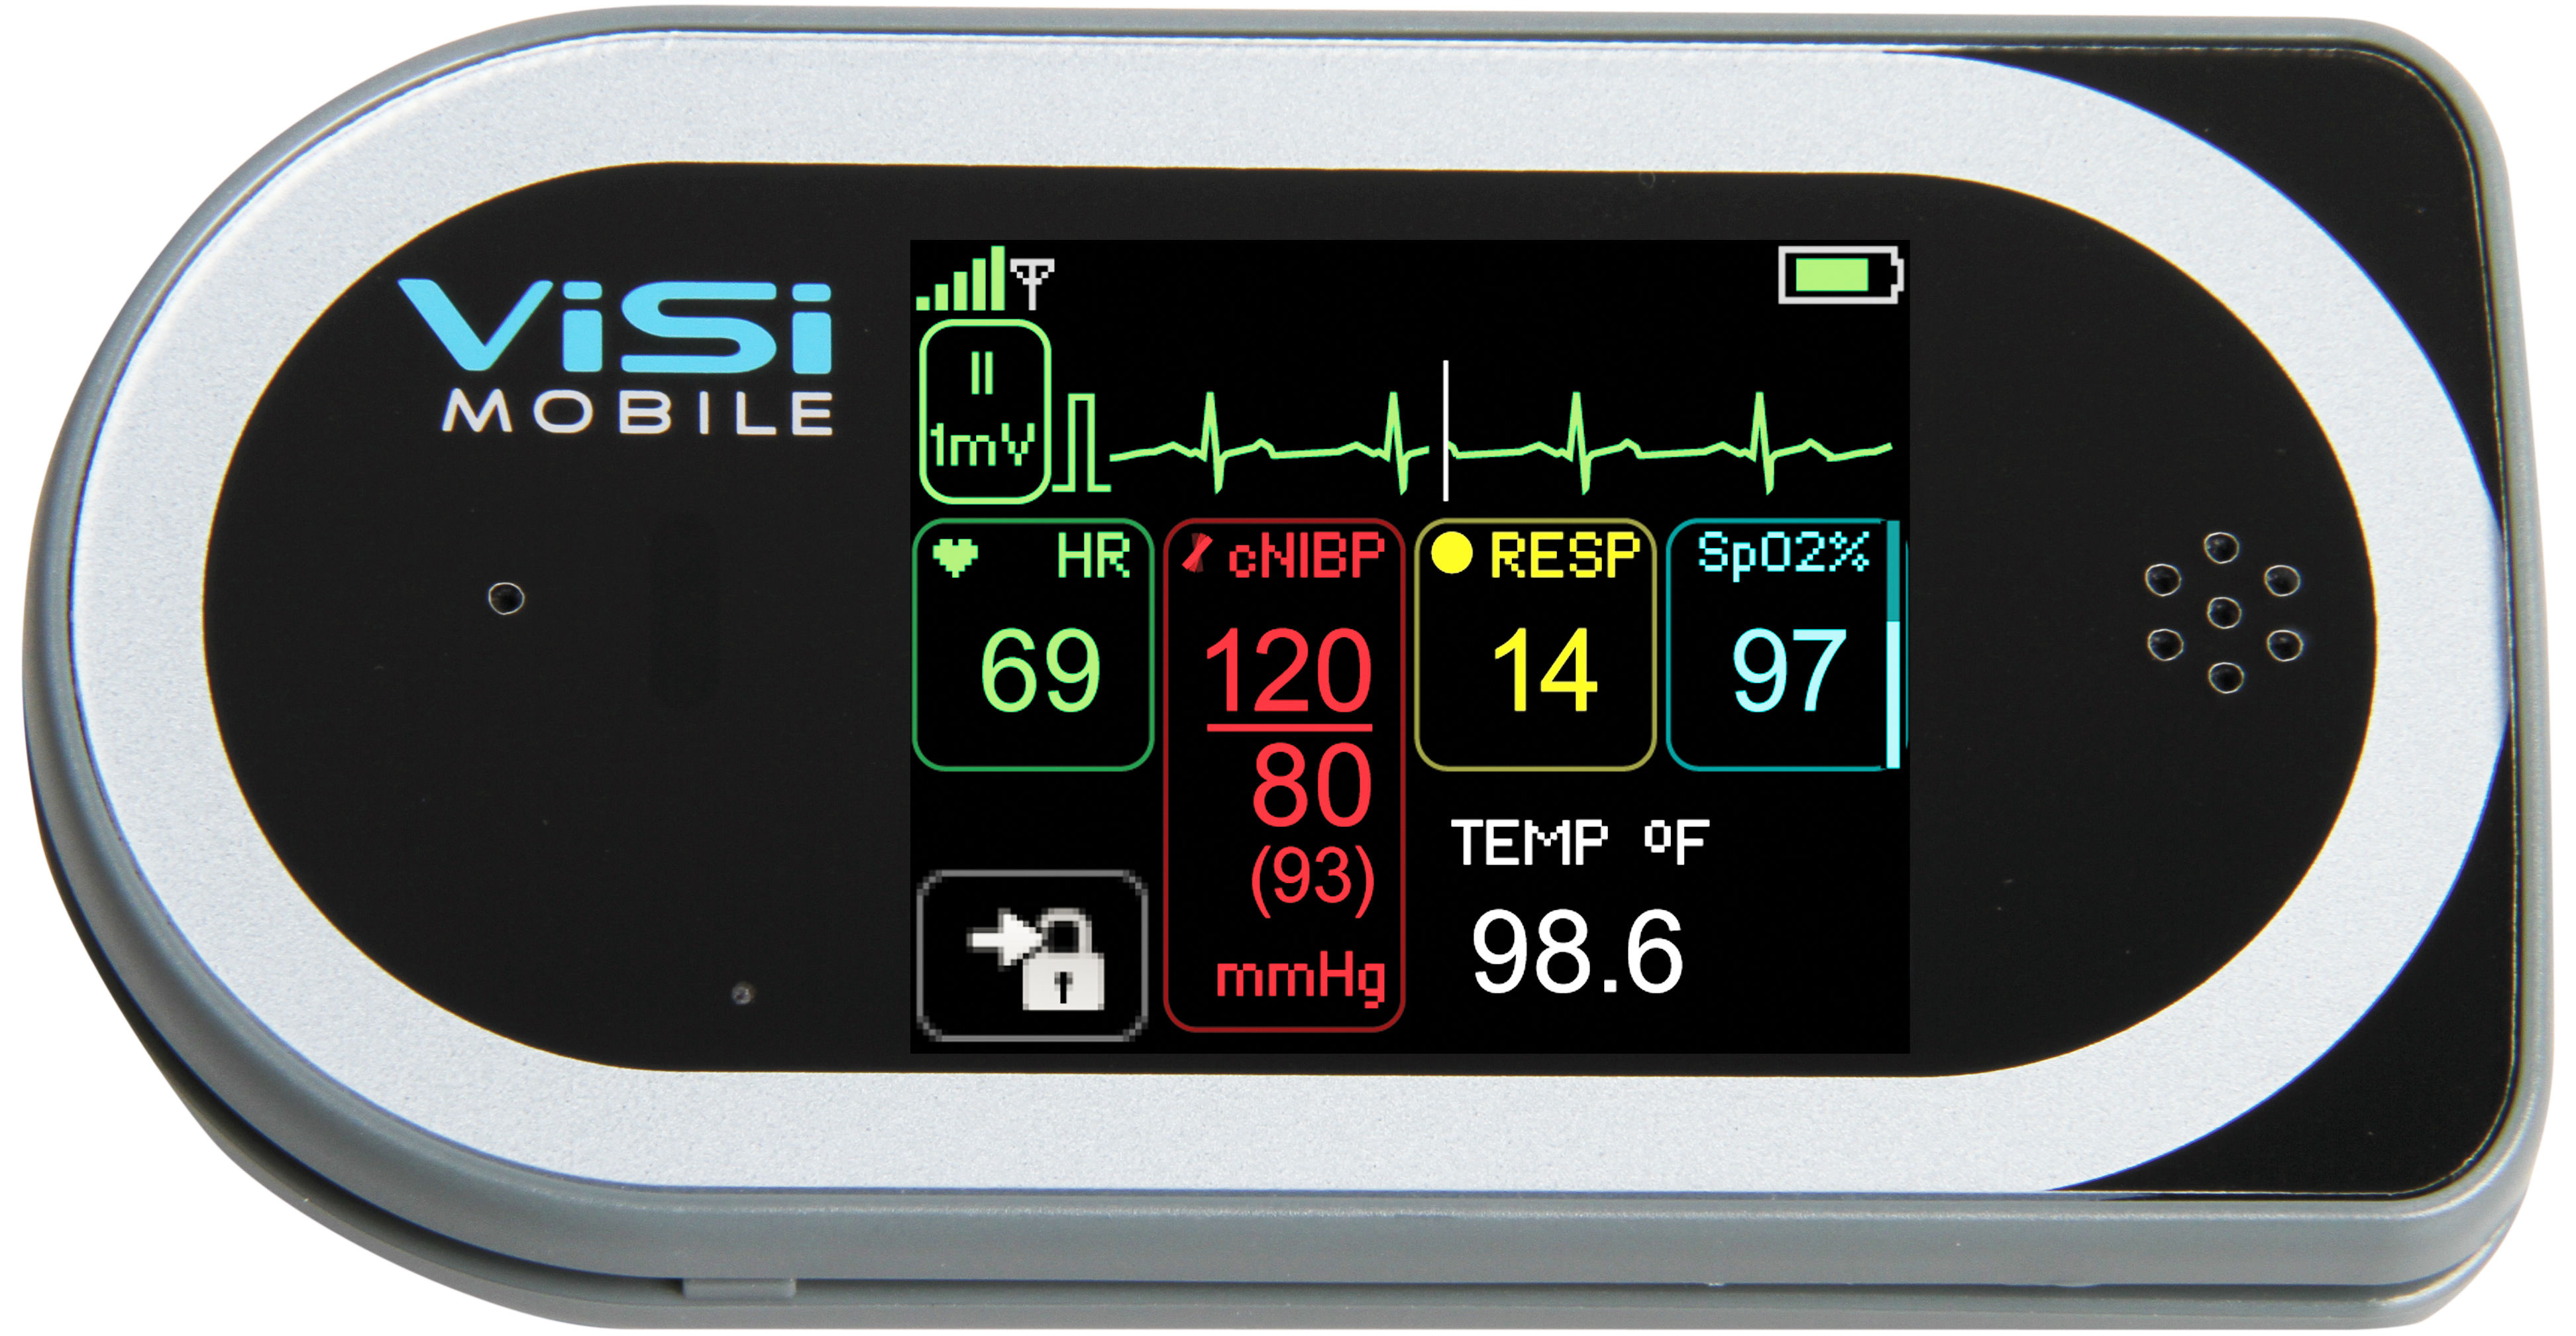
\includegraphics[scale=0.3]{figuras/estadoarte/visi/visi.jpg}
	\caption{Interfaz de usuario ViSi Mobile\textregistered}
	\label{visi1}
\end{figure}

Se puede observar en la figura \ref{visi1} la interfaz que puede ver el paciente al utilizar el dispositivo.

\begin{figure}[H]
	\centering
	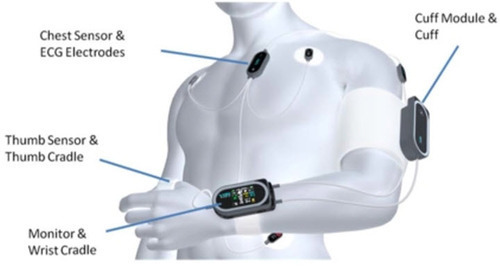
\includegraphics[scale=0.7]{figuras/estadoarte/visi/wear.jpg}
	\caption{Modo de uso ViSi Mobile\textregistered}
	\label{visi2}
\end{figure}

En la imagen de la figura \ref{visi2} se puede observar los sensores conectados al cuerpo que convergen al dispositivo que toma las señales.

\section{Qardiocore\textregistered}

QardioCore\cite{qardio} es un monitor de electrocardiograma inalámbrico diseñado para mejorar la detección y manejo de las condiciones cardíacas. Seis sensores se encargan de grabar y analizar sobre 20 millones de puntos de datos durante todo el día junto con otros signos vitales. Este dispositivo está orientado a personas con alto nivel de riesgo cardíaco causado por predisposición familiar, historial de ataques al corazón, presión alta, colesterol alto, diabetes o exceso de peso. Monitorea de forma precisa y continua la salud del corazón. El dispositivo graba datos de ECG, pulso, variación de pulso, temperatura corporal, ritmo respiratorio y niveles de estrés. A diferencia de los ECG tradicionales, QardioCore no utiliza gel ni cables para monitorear y funciona entre -20ºC y 60ºC. Adicionalmente es resistente al agua y su batería dura alrededor de un día. Respecto a las especificaciones técnicas, es capaz de funcionar con una frecuencia de 600 muestras por segundo y una resolución de 16 bit, apoyándose en comunicación Bluetooth 4.0 y plataforma exclusiva iOS (9.0 o superior)\cite{qardio_tel}.

\begin{figure}[H]
	\centering
	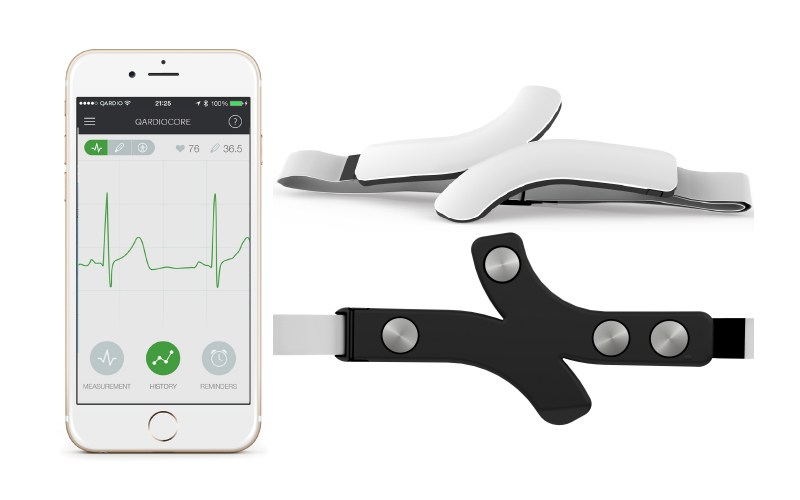
\includegraphics[scale=0.5]{figuras/estadoarte/qardio/qardio.jpg}
	\caption{Qardiocore multisensor}
	\label{qardio1}
\end{figure}

Se puede observar el dispositivo Qardiocore en la figura \ref{qardio1} que se conecta a un smartphone para mostrar los datos que se están tomando.

\newpage
Además como se muestra en la figura \ref{qardio2} es de simple uso, funciona como un cinturón en el pecho del paciente.

\begin{figure}[H]
	\centering
	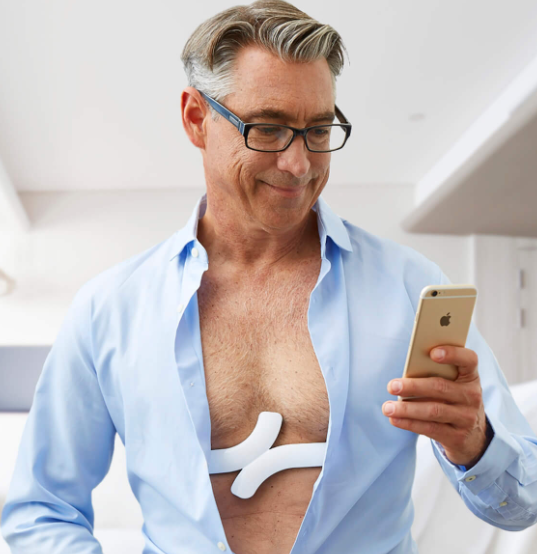
\includegraphics[scale=0.5]{figuras/estadoarte/qardio/wear.png}
	\caption{Modo de uso Qardiocore}
	\label{qardio2}
\end{figure}

\section{Nuubo\textregistered}

Nuubo\cite{nuubo} proporciona una nueva perspectiva en la monitorización cardiológica remota e inalámbrica. La plataforma de Nuubo, nECG platform, permite la captura del ECG dinámico a través de un innovador sistema que está basado en textiles biomédicos de nueva generación, y es rentable, remoto, continuo y no invasivo. Además, puede ser utilizado simultáneamente con uno o varios pacientes. Se basa en tecnología Bluetooth v2.0 + EDR (PC y móvil), con una frecuencia de 250 muestras por segundo y 12 bit de resolución\cite{nuubo_tel}.
La tecnología de electrodos textiles desarrollada por Nuubo simplifica enormemente los incómodos procedimientos tradicionales de conexión de electrodos, reduciéndolos al sencillo acto de vestir la camiseta nECG SHIRT que se muestra en la figura \ref{shirt}.

\begin{figure}[H]
	\centering
	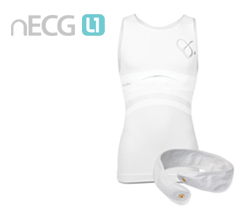
\includegraphics[scale=0.6]{figuras/estadoarte/nuubo/shirt.png}
	\caption{nECG Shirt}
	\label{shirt}
\end{figure}

El tejido elástico se adapta a los movimientos del paciente, quien puede realizar su actividad física diaria sin estar limitado por cables y sin necesidad de depender de personal médico especializado. Estas características junto con la información de contexto, la actividad física del paciente y su posición/postura, permite el desarrollo de un nuevo rango de soluciones y casos de uso. 

\begin{figure}[H]
	\centering
	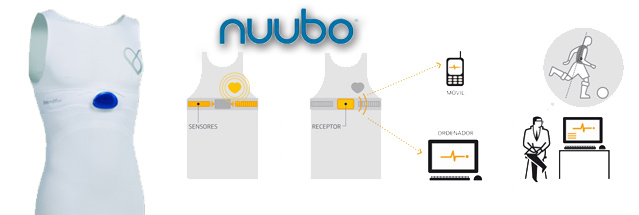
\includegraphics[scale=0.7]{figuras/estadoarte/nuubo/nuubo.png}
	\caption{Sistema Nuubo}
	\label{nuubo}
\end{figure}

Como se puede observar en la figura \ref{nuubo} la polera toma los datos que son enviados a un dispositivo movil o un computador para que sea visto por el doctor de manera remota.